\documentclass[11pt]{article}
\usepackage[margin=1in]{geometry}
\usepackage[T1]{fontenc}
\usepackage{amsmath,amssymb}
\usepackage{booktabs}
\usepackage{graphicx}
\usepackage[expansion=false]{microtype}
\usepackage[hidelinks]{hyperref}

\newcommand{\figorplaceholder}[2]{\IfFileExists{#1}{\includegraphics[width=\linewidth]{#1}}{\fbox{\parbox{0.9\linewidth}{\centering\vspace{1.2cm}#2\vspace{1.2cm}}}}}

\title{When Does Recalibration Blind a Streaming Anomaly Detector\\to a Persistent Shift, and How Can It Be Avoided?\\[0.3em]\large A pre-registered simulation study}
\author{{[Sabiha Khanum Z]}\\ {[Independent Researcher]}\\ \texttt{[khanum.z.sabiha@gmail.com]}}
\date{{[November 2026]} \quad (preprint, not peer reviewed)}

\begin{document}
\maketitle

\begin{abstract}
Streaming anomaly detectors usually keep updating their idea of ``normal'' so that they can follow drift. This causes a problem for persistent shifts. A shift is an anomaly at first, but if it lasts it becomes the new normal, so a detector that adapts quickly can absorb the shift before it has finished alerting. We test this in a pre-registered simulation. The stream is synthetic, with volatility clustering and tail weight matched to BTCUSDT 1-minute returns. A CUSUM detector with a rolling or periodically rebuilt baseline still alarms at least once almost as often as one with a fixed baseline (its detection probability drops only for windows of 100 bars or less), but its alert is much shorter. In the 500 bars after a one-sigma level shift, a baseline rebuilt every $W/4$ bars with $W=250$ keeps the alert on for 16\% as long as a fixed baseline, and a rolling window of 100 bars for 21\%. A simple absorption model predicts this well (mean absolute error 0.05 in alert coverage over 12 cells; Spearman 0.99). A drift-gated update holds the baseline while the alert is active and re-baselines afterwards. It closes at least 94\% of the coverage gap in all 19 shortened cells with the stricter two-level gate, and at least 66\% with the one-level gate. It keeps false alarms near their target rate and still tracks a benign drift. An Isolation Forest whose threshold is re-derived from recent scores shows the same effect: its alert covers 29\% to 42\% of what a frozen forest's covers, with no loss of detections. The study is synthetic and covers one stream family and one kind of shift. We report what failed as well as what held.
\end{abstract}

\section{Introduction}

Anomaly detectors on streams face a trade-off. Data drift, so a detector that never updates its baseline will raise false alarms as the world changes. But a detector that updates all the time may stop alarming just when something has really and lastingly changed. After a persistent shift, the behaviour we want is \emph{alert, hold, then re-baseline}. The shift should be reported, the baseline should not be allowed to move toward it while it is being reported, and only afterwards should the detector accept the new level as normal.

This paper asks when recalibration breaks that behaviour. We call a detector \emph{blind} to a shift if it raises no alert, or an alert too short to act on. We make four claims and test them with a pre-registered protocol: (C1) recalibration shortens or removes the alert on a persistent shift at a matched false-alarm rate; (C2) a simple model predicts when this happens; (C3) a drift-gated update restores the alert without giving up adaptation; and (C4) real data show the same pattern. C4 (a BTCUSDT 2022 illustration) is left for a later version. Here, real data are used only to match the simulated stream.

\section{Related work}

\paragraph{Change and drift detection.} The CUSUM test \cite{page1954,hawkins1998} is the classical way to catch a shift in a mean, and its behaviour is well understood, which is why we use it as the main detector. The concept drift literature \cite{gama2014survey,lu2019review} and windowing methods such as ADWIN \cite{bifet2007adwin} treat drift as something to detect and then adapt to. Hinder et al.\ \cite{hinder2024} survey unsupervised drift detection for monitoring, where the goal is to notice a change rather than follow it. The SPOT and DSPOT detectors \cite{siffer2017spot} set thresholds from extreme value theory and re-estimate them as the stream moves. This is the kind of adaptation we study, although we do not test those detectors here.

\paragraph{Streaming anomaly detection under drift.} Cao et al.\ \cite{cao2025} review streaming detectors and benchmark nine of them on synthetic streams with different drift types. They point out that most methods pair a detector with a model-update rule, and that ranking scores over a whole stream gives a misleading picture when the model is being updated. Our choice to match detectors on false-alarm rate comes from the same concern. A newer line of deep methods adapts to drift by pooling or switching models \cite{yoon2022arcus}, by adapting parameters online \cite{zhu2023meter}, or by test-time adaptation \cite{kim2026candi}. The paper closest to ours in spirit is AnDri \cite{park2025andri}. It notes that anomaly detection and drift detection are usually studied separately, and it keeps a set of normal patterns that can be switched on and off so that recurring anomalies are not simply absorbed as normal. AnDri works on subsequence anomalies and reports accuracy on real datasets. We look at a simpler setting, a level shift in a point-wise stream, and measure one thing: how long the alert stays on after the shift.

\paragraph{Evaluation.} Streaming benchmarks such as NAB \cite{lavin2015nab} score how early a detector fires, and larger comparisons \cite{schmidl2022eval,boniol2024decade} score detection accuracy over labelled data. A detector can fire early and still drop the alert quickly, and accuracy scores do not show this. Alert coverage after onset, which we use here, is meant to fill that gap.

Our contribution is narrow. We give a controlled, pre-registered measurement of how much of an alert survives baseline adaptation, and we test one simple remedy.

\section{Setup}

\paragraph{Stream.} Each stream has $N=20{,}000$ bars. The first 3{,}000 bars are a warm-up, and the fixed baseline is estimated from them. A persistent level shift of $+\delta$ unconditional standard deviations starts at an onset drawn uniformly from bars 6{,}000 to 12{,}000. The noise is a two-component GARCH(1,1) \cite{bollerslev1986,engle1999} with Student-$t$ innovations,
\[
\sigma_t^2 = v^{(1)}_t + v^{(2)}_t,\qquad v^{(i)}_{t+1} = w_i + a_i r_t^2 + b_i v^{(i)}_t,
\]
with fast component $(a_1,b_1)=(0.121,0.722)$, slow component $(a_2,b_2)=(0.0226,0.955)$, $\nu=5.26$, and $w_1,w_2$ chosen so that the total unconditional variance is one. A single GARCH(1,1) could not reproduce the real data (see Section~\ref{sec:deviations}), so we used two components.

We fitted the parameters to the monthly means (January to June 2022, 260{,}634 returns) of four scale-free statistics of BTCUSDT 1-minute log returns: $(q_{99}-q_1)/\mathrm{IQR}$ (6.67), $(q_{99.9}-q_{0.1})/\mathrm{IQR}$ (13.99), and the autocorrelation of $|r|$ at lags 1 and 60 (0.33 and 0.17). On long simulated streams the fitted generator gives 6.6, 15.3, 0.36 and 0.19. The extreme-tail ratio is too high (15.3 against 13.99). Intraday seasonality and jumps are not modelled.

\paragraph{Detector.} The main detector is a one-sided CUSUM on the standardised value $u_t=(x_t-m_t)/s_t$, with allowance $k=0.5$. Here $(m_t,s_t)$ is the baseline of the policy in use. The threshold is calibrated separately for every detector, policy and window, so that the in-control alarm-episode rate is 1 per 1{,}000 bars with the policy active (120 calibration streams and 120 independent check streams of 20{,}000 bars). Flags at most 5 bars apart form one alert episode.

\paragraph{Baseline policies.}
\begin{itemize}
\item \emph{Static}: the baseline is fixed at the end of the warm-up.
\item \emph{Rolling}($W$): mean and standard deviation of the last $W$ bars.
\item \emph{Periodic}($W$): the rolling baseline is recomputed every $W/4$ bars, and the CUSUM accumulator is reset at that point.
\item \emph{Gated-1L}: rolling, but the baseline is frozen when the alarm level is crossed and held for up to $K$ bars.
\item \emph{Gated-2L}: as gated-1L, plus a lower watch level (calibrated to 1 episode per 100 bars) that also freezes the baseline. A hold ends after $K$ bars, or earlier after 50 consecutive quiet bars. The baseline is then re-estimated from recent data.
\end{itemize}
$K=1000$ is the primary gate and $K=250$ is secondary. The window grid is $W\in\{50,100,250,500,1000,4000\}$.

\paragraph{Metrics.} The \emph{first episode} is the first alert episode that starts at or after the onset. Flags chained to an alert already in progress at onset are skipped and counted as ``contaminated''. $P(\text{detect})$ is the probability that a first episode occurs within a horizon of $H=500$ bars. A stream is \emph{blind} if there is no such episode, or if it lasts fewer than $D_{\min}=10$ bars. \emph{Alert coverage} is the fraction of the $H=500$ bars after onset that are in alert. The primary endpoint is the coverage of a policy divided by the coverage of the static baseline.

\paragraph{Absorption model.} Suppose a shift has lasted $s$ bars and the window holds $W$ bars. Then a fraction $p=s/W$ of the window is post-shift, so the baseline mean has moved by $p\delta$ and the baseline variance has become $1+p(1-p)\delta^2$. Once the baseline has absorbed enough of the shift, CUSUM can no longer see it. This happens at about $p^\ast\approx 0.44$ for $\delta=1$ and $0.66$ for $\delta=2$. We evaluate the model on a Gaussian ``model stream'' that follows this absorption path, with thresholds calibrated on iid noise.

\paragraph{Statistics.} Coverage ratios use a paired one-sided Wilcoxon signed-rank test (zero-split) against static. The 12 primary comparisons are adjusted with Holm's method \cite{holm1979}, and we give 95\% paired-bootstrap intervals (10{,}000 resamples). $P(\text{detect})$ uses the exact McNemar test. Trends in $W$ use a logistic GEE and a within-seed permutation test.

\paragraph{Isolation Forest.} The forest \cite{liu2008iforest} uses four features: the current value, and the mean, standard deviation and range over the last 30 bars. It is trained on the last $T\in\{500,1000,1500\}$ bars and refitted every $T/4$ bars. Its threshold is the 1\% quantile of the out-of-sample scores of the most recent $T/4$ bars. The frozen comparator is trained once on the warm-up, and its threshold is calibrated to the same in-control episode rate as the adaptive forest. This rate cannot be set to 1 per 1{,}000, because a quantile of $T/4$ scores cannot go below their minimum. At $q=0.01$ both forests raise 8 to 12 episodes per 1{,}000 bars.

\paragraph{Pre-registration.} The hypotheses, metrics, seeds and analysis plan are in a protocol tagged (\texttt{prereg-v1}) in the public repository before the test run. Development used seeds 1--30. The test used seeds 101--300 (100--200 for the forest) and was run once.

\section{Results}

\subsection{Recalibration seldom prevents the first alarm (H1a, negative)}

Detection is hardly affected except for small windows (Table~\ref{tab:detect}). Rolling $W=50$ and periodic $W=50$ and $100$ detect significantly less often than static (Holm $p<0.02$), but no cell loses half of the static detection rate. The pre-registered detection hypothesis H1a therefore fails. For windows of 250 and above, detection rates are within 1.5 percentage points of static.

\begin{table}[t]
\centering
\caption{$P(\text{detect})$ within 500 bars, level shift $\delta=1$, 200 test seeds. Static: 0.965.}
\label{tab:detect}
\begin{tabular}{lcccccc}
\toprule
$W$ & 50 & 100 & 250 & 500 & 1000 & 4000\\
\midrule
Rolling & 0.870 & 0.965 & 0.950 & 0.960 & 0.970 & 0.965\\
Periodic & 0.720 & 0.880 & 0.955 & 0.965 & 0.975 & 0.975\\
\bottomrule
\end{tabular}
\end{table}

\subsection{The alert is much shorter (H1a$'$)}

The alert, however, does not stay on (Table~\ref{tab:cov}). At $\delta=1$ the static baseline covers 94\% of the 500 bars after the shift. Rolling baselines with $W\le100$ and periodic baselines with $W\le500$ cover at most half of that, with Holm-adjusted $p<10^{-28}$ in each of these cells.

The practical claim holds. Periodic recalibration with $W=250$ and $W=500$, window sizes a deployed pipeline might well use, covers 16\% and 43\% of static's coverage. A rolling window with $W=250$ is clearly reduced (ratio 0.58, interval 0.55 to 0.61), though not by half at $\delta=1$. At $\delta=0.75$ it is (0.43). Windows of 1000 and above change the coverage little. Excluding events that start with an alert already in progress changes none of these conclusions. The effect also grows for smaller shifts (second column of Table~\ref{tab:cov}).

\begin{table}[t]
\centering
\caption{Alert coverage of the policy divided by that of the static baseline (95\% paired-bootstrap interval), 200 test seeds. Static coverage is 0.940 ($\delta=1$) and 0.877 ($\delta=0.75$). Bold: ratio $\le 0.5$ and Holm $p<0.05$.}
\label{tab:cov}
\begin{tabular}{llcc}
\toprule
Policy & $W$ & $\delta=1$ & $\delta=0.75$\\
\midrule
Rolling & 50 & \textbf{0.086} [0.077, 0.095] & \textbf{0.058} [0.050, 0.066]\\
 & 100 & \textbf{0.213} [0.197, 0.229] & \textbf{0.147} [0.132, 0.163]\\
 & 250 & 0.581 [0.548, 0.613] & \textbf{0.433} [0.397, 0.469]\\
 & 500 & 0.943 [0.903, 0.982] & 0.827 [0.771, 0.884]\\
 & 1000 & 0.984 [0.952, 1.016] & 0.966 [0.914, 1.018]\\
 & 4000 & 0.999 [0.972, 1.026] & 1.006 [0.963, 1.049]\\
\midrule
Periodic & 50 & \textbf{0.009} [0.008, 0.010] & \textbf{0.007} [0.005, 0.008]\\
 & 100 & \textbf{0.037} [0.033, 0.041] & \textbf{0.027} [0.023, 0.030]\\
 & 250 & \textbf{0.162} [0.151, 0.173] & \textbf{0.120} [0.109, 0.131]\\
 & 500 & \textbf{0.425} [0.403, 0.448] & \textbf{0.342} [0.316, 0.369]\\
 & 1000 & 0.795 [0.761, 0.828] & 0.695 [0.652, 0.739]\\
 & 4000 & 0.977 [0.951, 1.004] & 0.962 [0.920, 1.006]\\
\bottomrule
\end{tabular}
\end{table}

\begin{figure}[t]
\centering
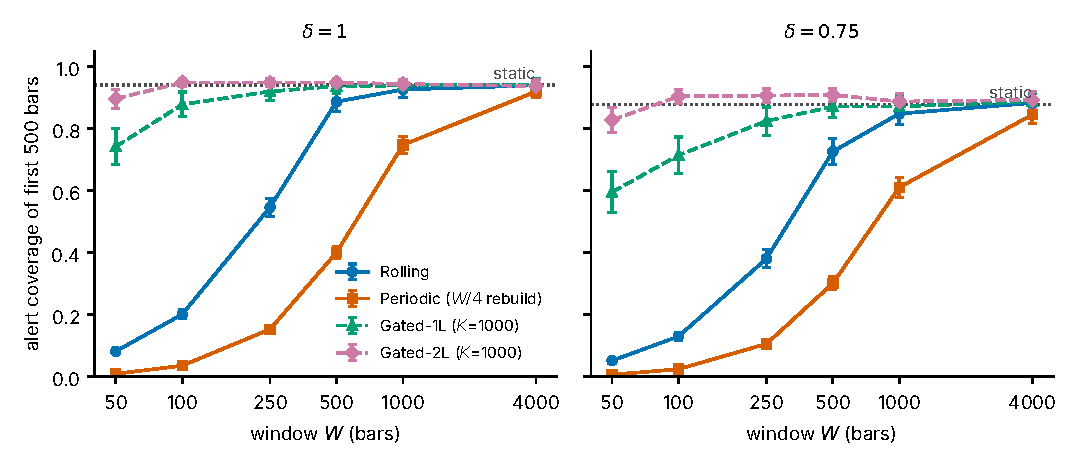
\includegraphics[width=\linewidth]{fig_coverage.pdf}
\caption{Mean alert coverage of the first 500 bars after a level shift against window size $W$, 200 test seeds, error bars 95\% intervals over seeds. Dotted line: static baseline. Dashed lines: gated policies with $K=1000$.}
\label{fig:cov}
\end{figure}

\subsection{Dependence on the window (H1b, H1c)}

The longer the window, the more often the shift is detected, and the less often it is blind within the first 200 bars. More of those bars are also in alert. Every permutation test for rolling and periodic baselines at $\delta=0.75$ and $\delta=1$ has $p\le 10^{-4}$. At $\delta=2$ the rolling trends are not significant, because nearly every shift is detected (a ceiling effect). The periodic trends stay significant ($p\le0.002$).

\subsection{A simple model predicts the effect (H2b)}

On the 12 level cells the absorption model agrees with the simulation (Table~\ref{tab:model}). Both pre-registered criteria are met (mean absolute error $\le0.10$ and Spearman correlation $\ge0.8$). The largest gaps are at small $W$. For rolling $W=50$ the model predicts $P(\text{blind})=0.46$ against 0.28 in the simulation, and a mean alert of 18 bars against 39. The model misses this because it ignores that clustered volatility makes real alerts longer. For larger windows the model is too optimistic about periodic baselines (0.85 predicted against 0.75 simulated at $W=1000$).

\begin{table}[t]
\centering
\caption{Agreement between the model stream and the simulation, 12 level cells, 200 test seeds. Criteria: MAE $\le0.10$, Spearman $\ge0.80$.}
\label{tab:model}
\begin{tabular}{lcc}
\toprule
Quantity & MAE & Spearman\\
\midrule
$P(\text{blind})$ & 0.031 & 0.88\\
Alert coverage & 0.050 & 0.99\\
\bottomrule
\end{tabular}
\end{table}

\subsection{A drift-gated update restores the alert (H3)}

Table~\ref{tab:gate} compares the gates with the baselines they gate, at $K=1000$ and $\delta=1$. In all 19 shortened cells (the union of cells flagged in development and by the model stream) the one-level gate closes at least 66\% of the coverage gap between the reference policy and static, and the two-level gate at least 94\%. The two-level gate also recovers at least 90\% of static's detection rate in every cell.

With $K=250$ no gate meets the half-gap criterion. This is expected: the horizon is 500 bars, so the hold is released inside it and coverage is capped near $K/H$. We therefore use $K=1000$ as the primary setting. This criterion is partly definitional, so it should be read together with the checks below.

\begin{table}[t]
\centering
\caption{Alert coverage of the gated policies ($K=1000$) against the policy they gate, $\delta=1$, 200 test seeds. Static: 0.940.}
\label{tab:gate}
\begin{tabular}{llccc}
\toprule
Policy & $W$ & Reference & Gated-1L & Gated-2L\\
\midrule
Rolling & 50 & 0.081 & 0.741 & 0.895\\
 & 100 & 0.200 & 0.877 & 0.949\\
 & 250 & 0.546 & 0.919 & 0.948\\
Periodic & 50 & 0.008 & 0.741 & 0.895\\
 & 100 & 0.035 & 0.877 & 0.949\\
 & 250 & 0.152 & 0.919 & 0.948\\
 & 500 & 0.400 & 0.936 & 0.948\\
\bottomrule
\end{tabular}
\end{table}

\paragraph{False alarms (H3b).} With the gate active, the in-control episode rate on independent check streams is between 0.95 and 1.08 per 1{,}000 bars in all level-statistic cells.

\paragraph{Cost of the hold (H3c, H3d).} The one-level gate is frozen for about 5\% to 6\% of in-control bars and updates its baseline about 940 to 950 times per 1{,}000 bars. The two-level gate is frozen for 37\% to 51\% of in-control bars and updates 490 to 630 times per 1{,}000 bars. It gives up about half of the adaptation in return for a stricter hold. Periodic baselines update far less often (about 1 to 83 per 1{,}000) but are the most affected by absorption.

\paragraph{Benign drift (H3f).} On a benign level ramp of 5{,}000 bars, the static baseline is in alert for 75\% of the ramp, against 2.5\% on a stationary control. The two-level gate stays at 2.6\% to 3.8\% at every window (control 1.6\% to 2.5\%). Rolling baselines with $W\le1000$ stay at 0.5\% to 2.8\%. Rolling $W=4000$ lags behind the ramp and is in alert for 70\% of it. During the ramp the gate raises 1.25 to 1.82 episodes per 1{,}000 bars, against about 1 in control.

\paragraph{Limit of the horizon metric.} Coverage is measured over 500 bars, but the hold lasts up to 1{,}000. The metric therefore cannot tell holding from holding and then re-baselining correctly. The re-baselining step was meant to be checked with a rebound metric on 200-bar transient shifts (H3e), which is not part of this study.

\subsection{An Isolation Forest shows the same effect (H1e)}

We re-derive the forest's threshold from recent out-of-sample scores. Its alert then covers 29\% to 42\% of the frozen forest's coverage in all six cells (Table~\ref{tab:if}; Holm $p<10^{-4}$ in each cell). The adaptive forest detects at least as often as the frozen one in every cell (+8 to +25 percentage points). An unmatched sensitivity comparison, with the frozen forest at the same quantile rather than the same episode rate, gives ratios of 0.29 to 0.41 and the same conclusion.

\begin{table}[t]
\centering
\caption{Isolation Forest: alert coverage of the adaptive forest and of the frozen forest matched on in-control episode rate, 100 test seeds. $\Delta P$: adaptive minus frozen $P(\text{detect})$.}
\label{tab:if}
\begin{tabular}{ccccccc}
\toprule
$\delta$ & Train $T$ & Adaptive & Frozen & Ratio & $\Delta P$\\
\midrule
0.75 & 500 & 0.141 & 0.464 & 0.30 & +0.18\\
0.75 & 1000 & 0.172 & 0.408 & 0.42 & +0.25\\
0.75 & 1500 & 0.191 & 0.562 & 0.34 & +0.10\\
1.0 & 500 & 0.148 & 0.515 & 0.29 & +0.19\\
1.0 & 1000 & 0.187 & 0.450 & 0.42 & +0.20\\
1.0 & 1500 & 0.207 & 0.605 & 0.34 & +0.08\\
\bottomrule
\end{tabular}
\end{table}

\begin{figure}[t]
\centering
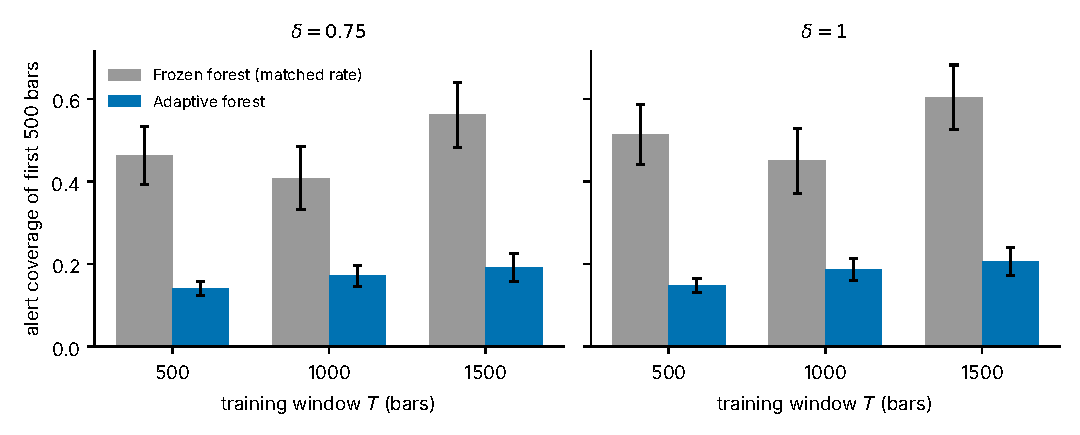
\includegraphics[width=\linewidth]{fig_if.pdf}
\caption{Isolation Forest: alert coverage of the first 500 bars after the shift, adaptive forest against the frozen forest matched on in-control episode rate (100 test seeds, 95\% intervals).}
\label{fig:if}
\end{figure}

\section{Decisions made after seeing the development data}\label{sec:deviations}

We revised the protocol during development, before the test run. The revisions are recorded in the protocol and the repository. The main ones are:
\begin{itemize}
\item The primary endpoint is alert coverage (H1a$'$), because the detection-rate version (H1a) failed on development data by a wide margin. We keep H1a and report it as a negative result.
\item $K=1000$ is the primary gate, because $K=250$ cannot meet the coverage criterion with a 500-bar horizon.
\item We added the Isolation Forest check (H1e) after seeing development results.
\item We changed the generator from a single GARCH(1,1) to the two-component form. The single model could not reproduce the real data. Its best fit gave $(q_{99}-q_1)/\mathrm{IQR}$ of 4.8 against 7.0 and a lag-60 autocorrelation of $|r|$ of 0.005 against 0.21. The targets are monthly means, because the pooled statistics are inflated by month-to-month changes in volatility.
\item We dropped the variance-shift statistic from the confirmatory analysis. On this stream a static baseline spends 57\% to 60\% of in-control bars in alert at the matched episode rate, so the statistic is not usable. This cut the primary family from 24 to 12 comparisons, which makes the Holm correction less strict. The affected development $p$-values were below $10^{-5}$, so the conclusions do not depend on this change.
\item We restricted the model-agreement test (H2b) to the level cells, for the same reason. Over the 24 cells that included the variance statistic, it fails on development data (coverage MAE 0.126), because the Gaussian model overpredicts detection of variance shifts. We made this restriction after seeing that result.
\end{itemize}

\section{Limitations}

This is a simulation. The stream matches four robust statistics of BTCUSDT returns, but not intraday seasonality, jumps or the extreme tail (the tail ratio is too high). On the confirmatory seeds we tested only a one-sided level shift with a CUSUM detector, plus an Isolation Forest for one comparison. We did not test variance shifts, other detectors (EWMA, z-score, DSPOT-style, ADWIN-triggered recalibration) or transient shifts. The real-data illustration (C4) is left for later.

The gated policies were chosen and tuned on the same stream family, and the 500-bar horizon cannot test the re-baselining step. The two-level gate adapts about half as often as the one-level gate. The Isolation Forest runs at about 8 to 12 alarm episodes per 1{,}000 bars, roughly ten times the CUSUM rate, and the matching of the frozen forest's rate was loose for $T=1500$ (calibrated 8.0, check 11.5 per 1{,}000). Several analysis choices were fixed after we saw development data (Section~\ref{sec:deviations}), although the test seeds were not touched until the protocol was frozen.

\section{Conclusion}

On a stream matched to BTCUSDT 1-minute returns, recalibrating the baseline does not usually stop a CUSUM detector from alarming, but it cuts the alert to a fraction of what a fixed baseline gives. For a periodically rebuilt baseline with $W=250$ the alert is about six times shorter. A model of window absorption predicts which settings are affected. Holding the baseline while an alert is active, then re-baselining, restores most of the alert. In the settings we tested it does not disturb the false-alarm rate or the tracking of benign drift. The same shortening appears in an Isolation Forest with a re-derived threshold. These results come from simulation and need to be replicated on real streams and other detectors before anyone relies on them.

\section*{Reproducibility}
Code, protocol and the frozen tag are in the repository \texttt{adaptive-baseline-blindness} (tag \texttt{prereg-v1}; commit hash in \texttt{FREEZE.md}). [Add the public URL and archive DOI here.] Seeds: development 1--30, test 101--300 (forest 101--200), calibration 12345 and 54321, bootstrap 2026.

\begin{thebibliography}{99}
\bibitem{page1954} E.~S. Page. Continuous inspection schemes. \emph{Biometrika}, 41(1/2):100--115, 1954.
\bibitem{hawkins1998} D.~M. Hawkins, D.~H. Olwell. \emph{Cumulative Sum Charts and Charting for Quality Improvement}. Springer, 1998.
\bibitem{gama2014survey} J.~Gama, I.~\v{Z}liobait\.{e}, A.~Bifet, M.~Pechenizkiy, A.~Bouchachia. A survey on concept drift adaptation. \emph{ACM Computing Surveys}, 46(4), 2014.
\bibitem{lu2019review} J.~Lu, A.~Liu, F.~Dong, F.~Gu, J.~Gama, G.~Zhang. Learning under concept drift: A review. \emph{IEEE Transactions on Knowledge and Data Engineering}, 31(12):2346--2363, 2019.
\bibitem{bifet2007adwin} A.~Bifet, R.~Gavald\`a. Learning from time-changing data with adaptive windowing. In \emph{Proc.\ SIAM International Conference on Data Mining}, 2007.
\bibitem{siffer2017spot} A.~Siffer, P.-A. Fouque, A.~Termier, C.~Largou\"et. Anomaly detection in streams with extreme value theory. In \emph{Proc.\ ACM SIGKDD}, 2017.
\bibitem{hinder2024} F.~Hinder, V.~Vaquet, B.~Hammer. One or two things we know about concept drift: a survey on monitoring in evolving environments. Part A: detecting concept drift. \emph{Frontiers in Artificial Intelligence}, 7:1330257, 2024.
\bibitem{cao2025} Y.~Cao, Y.~Ma, Y.~Zhu, K.~M. Ting. Revisiting streaming anomaly detection: benchmark and evaluation. \emph{Artificial Intelligence Review}, 58(1):8, 2025.
\bibitem{park2025andri} J.~Park, F.~Chiang, M.~Milani. Adaptive anomaly detection in the presence of concept drift. arXiv:2506.15831, 2025.
\bibitem{yoon2022arcus} S.~Yoon, Y.~Lee, J.-G. Lee, B.~S. Lee. Adaptive model pooling for online deep anomaly detection from a complex evolving data stream. In \emph{Proc.\ ACM SIGKDD}, pages 2347--2357, 2022.
\bibitem{zhu2023meter} J.~Zhu, S.~Cai, F.~Deng, B.~C. Ooi, W.~Zhang. METER: A dynamic concept adaptation framework for online anomaly detection. \emph{Proc.\ VLDB Endowment}, 17(4):794--807, 2023.
\bibitem{kim2026candi} H.~Kim, J.~Mok, H.~Lee, J.~Shin, S.~Yoon. CANDI: Curated test-time adaptation for multivariate time-series anomaly detection under distribution shift. In \emph{Proc.\ AAAI}, 40(17):15018--15026, 2026.
\bibitem{lavin2015nab} A.~Lavin, S.~Ahmad. Evaluating real-time anomaly detection algorithms: the Numenta Anomaly Benchmark. In \emph{Proc.\ IEEE ICMLA}, 2015.
\bibitem{schmidl2022eval} S.~Schmidl, P.~Wenig, T.~Papenbrock. Anomaly detection in time series: a comprehensive evaluation. \emph{Proc.\ VLDB Endowment}, 15(9):1779--1797, 2022.
\bibitem{boniol2024decade} P.~Boniol, Q.~Liu, M.~Huang, T.~Palpanas, J.~Paparrizos. Dive into time-series anomaly detection: a decade review. arXiv:2412.20512, 2024.
\bibitem{liu2008iforest} F.~T. Liu, K.~M. Ting, Z.-H. Zhou. Isolation forest. In \emph{Proc.\ IEEE ICDM}, pages 413--422, 2008.
\bibitem{bollerslev1986} T.~Bollerslev. Generalized autoregressive conditional heteroskedasticity. \emph{Journal of Econometrics}, 31(3):307--327, 1986.
\bibitem{engle1999} R.~F. Engle, G.~G.~J. Lee. A permanent and transitory component model of stock return volatility. In \emph{Cointegration, Causality, and Forecasting}, pages 475--497. Oxford University Press, 1999.
\bibitem{holm1979} S.~Holm. A simple sequentially rejective multiple test procedure. \emph{Scandinavian Journal of Statistics}, 6(2):65--70, 1979.
\end{thebibliography}
\end{document}